\chapter{Auswertung der Ergebnisse}
Insgesamt wurden einige Testreihen zur Stabilisierung des Laufverhaltens, zur Pfadplanung sowie zur Umsteuerung von Hindernissen durchgeführt.
Während die Stabilisierung erfolgreich durchgeführt wurde, zeigen insbesondere die Testreihen zur Pfadverfolgung, auf denen die Hindernisumsteuerung basiert, nicht die erwünschten Ergebnisse.
Zwar steuert der Roboter manchmal zielstrebig auf das DynamicTarget zu, allerdings ist sein Laufverhalten dabei stark instabil und die Aufgabe wird nicht verlässlich erfüllt.
Da die dabei verwendete Reward-Funktion und somit das gestellte Reinforcement Learning Problem fundamental sehr ähnlich zur Projektbasis \cite{waidner.2020} aufgebaut sind, ist die Ursache nur schwer zu bestimmen.

\autoref{fig:losses} stellt eine Übersicht der in \autoref{sec:bewertung} beschriebenen Bewertungskriterien für die einzelnen Trainingsdurchläufe dar.
Hierbei existieren einige Auffälligkeiten.
Die Kurve des Policy Loss sollte eigentlich im Laufe des Trainings abnehmen, wenn die Policy zu einer stabilen Funktion konvergiert.
\autoref{fig:losses} zeigt ein breites Spektrum, über das die verschiedenen Policy Losses verteilt liegen.
Auffällig ist dabei jedoch, dass die Losses zwar in der Regel einer starken Schwankung unterliegen, diese sich jedoch bis auf wenige Ausnahmen auf einen recht engen Wertebereich für jede Kurve beschränken.
Im Falle des Value Losses sollte der Wert zu Beginn hoch liegen und dann im Laufe des Trainings zu einem niedrigen Wert konvergieren.
Auch bei diesen Kurven können bei den meisten Trainingsdurchläufen hohe Schwankungen anstatt der gewünschten Konvergenz beobachtet werden.
Zwar gibt es auch einige Kurven, die grob dem erwarteten Verlauf entsprechen, jedoch konvergieren diese im Verhältnis zur Länge des Trainingsdurchlaufs viel zu früh.

Sowohl beim Policy als auch beim Value Loss kann beobachtet werden, dass einige Kurven sehr stabile und niedrige Werte aufweisen.
Diese Kurven entstanden nach der Korrektur der Hyperparameter, weshalb auf eine potenzielle Überkorrektur geschlossen werden kann.

Zwar würden fehlerhaft optimierte Hyperparameter und die Verläufe der Losses theoretisch die schlechten Trainingsergebnisse erklären, jedoch muss in diesem Zusammenhang auch darauf hingewiesen werden, dass die Stabilisierung des Laufverhaltens äußerst erfolgreich trainiert wurde, allerdings ebenso Verläufe der Losses zeigt, die eigentlich nicht zu einem erfolgreichen Training passen.
Dadurch wird die oben geübte Kritik infrage gestellt.

\begin{figure}
    \centering
    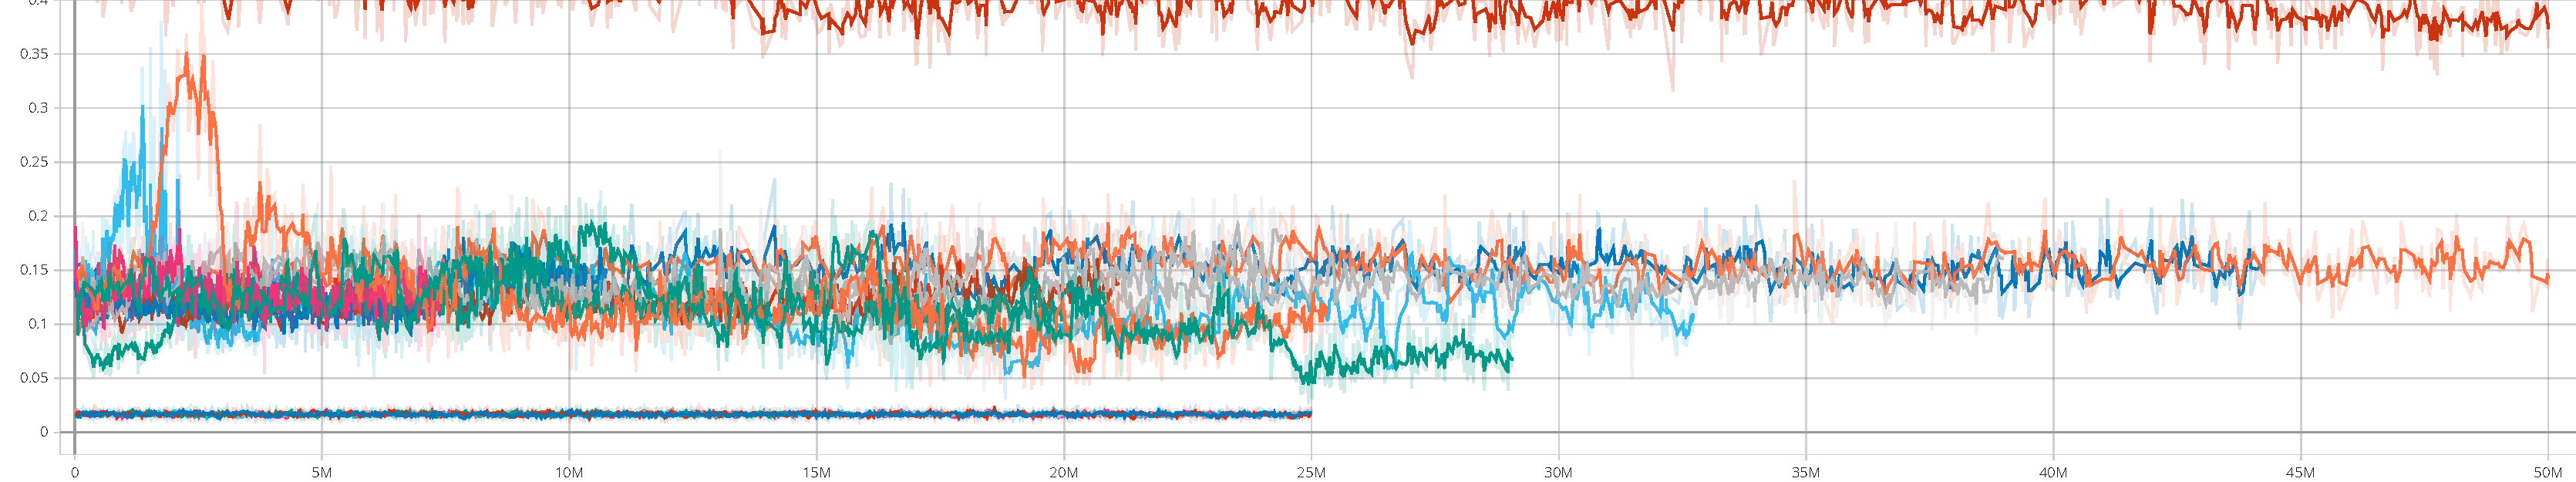
\includegraphics[width = \textwidth]{Bilder/ml-agents/Losses_Policy Loss.pdf}
    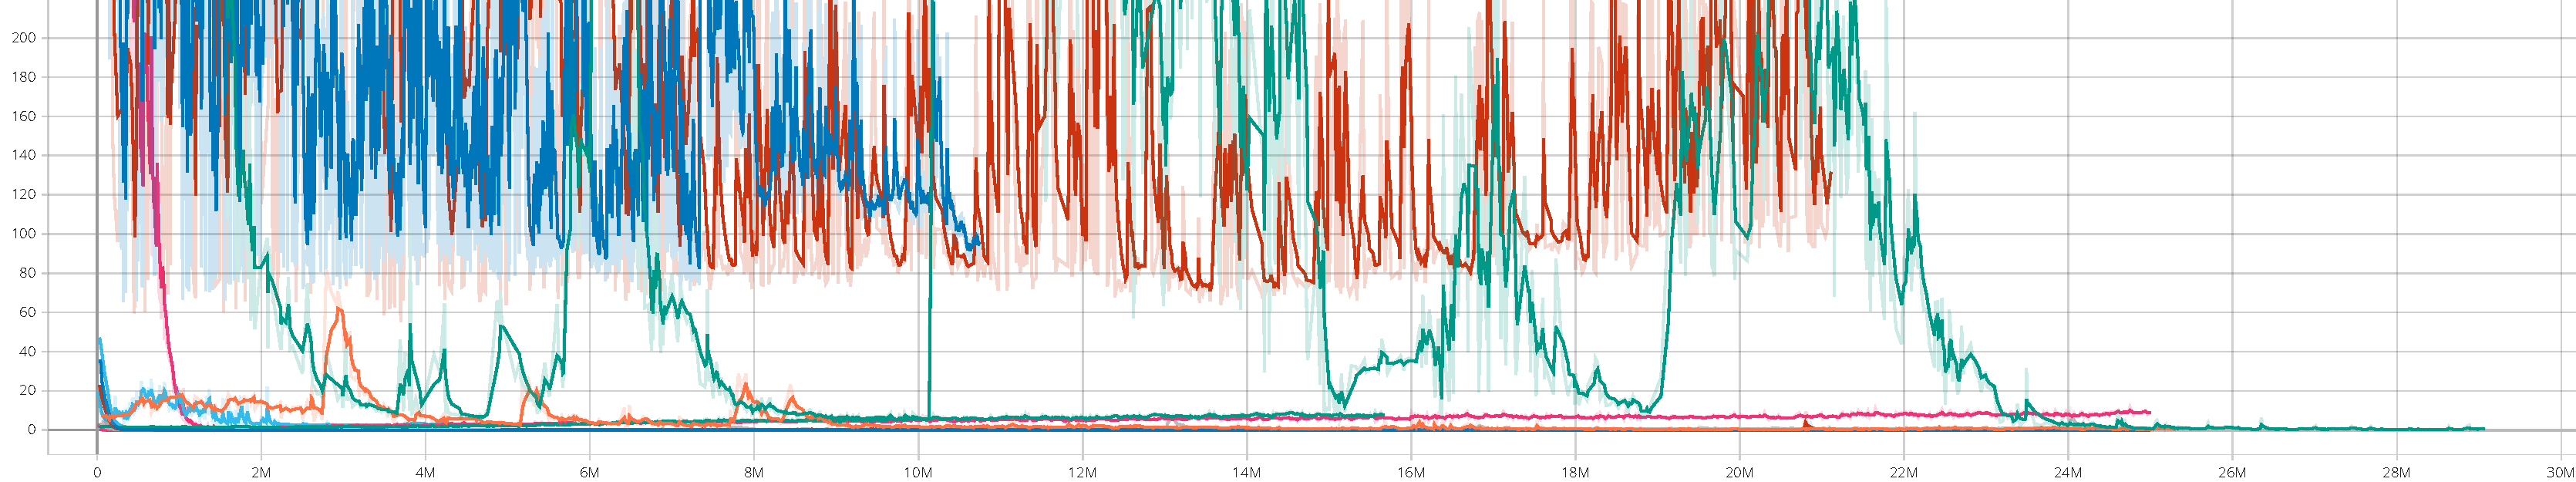
\includegraphics[width = \textwidth]{Bilder/ml-agents/Losses_Value Loss.pdf}
    \caption[Policy und Value Losses der Trainingsdurchläufe]{Policy Losses (oben) und Value Losses (unten) der Trainingsdurchläufe}
    \label{fig:losses}
\end{figure}

% \begin{itemize}
%     \item Unterschiede zu Crawler-Example
%     \item denkbar sind Fehler in der Simulation der Servomotoren, die zu einem unrealistischen Ergebnis führen
%     \item evaluieren, um welche Sensoren der Roboter in der Realität sinnvoll ergänzt werden könnte und dem Roboter mehr Informationen über sich selbst bereitstellen; Mangel an Informationen wurde hier als Grunddefinition gesetzt, ist jedoch elementarster Unterschied zu vergleichbaren Projekten, welche allerdings deutlich erfolgreichere Ergebnisse vorweisen
%     \item herausfinden, warum Policy Loss / Value Loss so hoch sind und wie das Training nachhaltig stabilisiert werden könnte
% \end{itemize}

\section{Future Work}
Als Future Work gilt es, die Fehlerquellen der aktuellen Problemstellung und Simulationsumgebung zu finden, um das implementierte Training erfolgreich und mit stabilem Ergebnis durchführen zu können.
Dafür können verschiedene Konfigurationen von Hyperparametern versucht werden, welche das Problem potenziell verringern oder lösen könnten.
Weiterhin dürfte es lohnenswert sein, ein Augenmerk auf die Unterschiede und Parallelen der vorliegenden Problemstellung zum wiederholt erwähnten Crawler-Example zu legen.
Allerdings dürfen auch fundamentale Unterschiede der beiden Szenarios nicht außer Acht gelassen werden, die eine direkte Übertragung unmöglich machen.
Primär sind dies die unterschiedliche Anzahl und Art der Gelenke genauso wie die zur Verfügung gestellten Eingabedaten.
Auch Fehler in der Simulation der Servomotoren können als Ursache nicht ausgeschlossen werden, da diese etwa das zielgenaue Koordinieren der Gelenke erschweren könnte und somit zwar zur Bewältigung einzelner Aufgaben genügt, jedoch der komplexer werdenden Problemstellung nicht mehr gewachsen ist.

Sollten mit den aufgelisteten Maßnahmen kein Erfolg erreicht werden, so könnte es auch interessant sein, den dezentralen Ansatz von Schilling et al. \cite{schilling2020decentralized} dediziert im Kontext der vorliegenden Problemstellung zu erforschen.

Ein elementarer Unterschied, der diese Arbeit von anderen abgrenzt, die dem State of the Art entsprechend, sind die stark beschränkten Eingabedaten.
Den Trainingsalgorithmen in vergleichbaren Projekten stehen bedeutend mehr Daten zu sich selbst und ihrer Umgebung zur Verfügung.
Deshalb wird der Schluss gezogen, dass wahrscheinlich sämtliche oben genannten Maßnahmen nur eine eingeschränkte Wirksamkeit entfalten können, solange die Sensorik des Roboters nicht erweitert wird.
Deshalb sollte zukünftig weiterhin evaluiert werden, mit welchen Sensoren der Roboter in der Realität sinnvoll ergänzt werden könnte, um dem Roboter hilfreiche Informationen über seinen eigenen Zustand zur Verfügung zu stellen.